% tikzify 利用マニュアル  (LuaLaTeX:  lualatex tikzify-manual.tex を2回)
% Copyright (c) 2026 Kosei Kawaguchi  -- MIT License (../LICENSE.md)
\documentclass[a4paper,11pt]{ltjsarticle}
\usepackage[margin=22mm]{geometry}
\usepackage{graphicx,adjustbox,booktabs,array,xcolor,fancyvrb,enumitem}
\usepackage{tikz,pgfplots,forest,tikz-cd,circuitikz}
\pgfplotsset{compat=1.18}
\usetikzlibrary{arrows.meta,positioning,shapes.geometric,shapes.misc,automata,quotes,
  angles,calc,decorations.pathmorphing,patterns.meta}
\usepackage[hidelinks]{hyperref}

\definecolor{ink}{HTML}{1F2430}
\definecolor{accent}{HTML}{C8102E}
\definecolor{codebg}{HTML}{F4F5F7}
\setlist{nosep,leftmargin=*}
\fvset{fontsize=\small,frame=single,framesep=6pt,rulecolor=\color{black!20}}
\newcommand{\cmd}[1]{\texttt{#1}}
\newcommand{\opt}[1]{\texttt{\detokenize{#1}}}
\renewcommand{\arraystretch}{1.25}

\title{\textbf{tikzify} 利用マニュアル\\[2pt]
  \large 図版を TikZ に起こして自分の文書へ挿入する Claude Code 用スキル}
\author{Kosei Kawaguchi}
\date{2026年10月}

\begin{document}
\maketitle
\tableofcontents
\bigskip

% ------------------------------------------------------------------
\section{概要}

tikzify は、手書きの図・スキャン・スクリーンショット・PDF / SVG / EPS の図版を
TikZ に起こし、自分の \LaTeX{} 文書へ \verb|\input| 1行で挿入できる形で納品するための
Claude Code 用スキルです。Claude Code に「この図を TikZ にして」と頼むと、
次の流れで作業が進みます。

\begin{center}
\begin{tikzpicture}[node distance=5mm and 7mm, >={Stealth[length=2mm]},
    stp/.style={draw, rounded corners=2mm, align=center, minimum height=11mm,
      text width=23mm, font=\small, fill=codebg},
    tag/.style={font=\scriptsize\ttfamily, text=accent}]
  \node[stp] (a) {図を読む\\[-1pt]\scriptsize 座標グリッド};
  \node[stp, right=of a] (b) {TikZ を書く\\[-1pt]\scriptsize 意図を清書};
  \node[stp, right=of b] (c) {原図と照合\\[-1pt]\scriptsize 重ね合わせ};
  \node[stp, right=of c] (d) {文書へ挿入\\[-1pt]\scriptsize 不足分だけ追記};
  \draw[->] (a) -- (b); \draw[->] (b) -- (c); \draw[->] (c) -- (d);
  \draw[->] (c.south) -- ++(0,-4mm) -| node[pos=0.25, below, font=\scriptsize]{ずれがあれば直す} (b.south);
  \node[tag, above=1mm of a] {grid.py / svg2tikz.py};
  \node[tag, above=1mm of c] {build.py / measure.py};
  \node[tag, above=1mm of d] {insert.py};
\end{tikzpicture}
\end{center}

手書きの線をそのままなぞるのではなく、描き手が意図した構造
(揃った位置、同じ大きさの箱、正しい記号、数式)を TikZ で組み直します。
出来上がった図は元の図と同じ縮尺で重ね合わせて確認し、
ずれがなくなるまで直してから納品します。

\subsection{納品物}
図1枚につき、次のファイルができます。

\begin{center}
\begin{tabular}{>{\ttfamily}l p{0.62\linewidth}}
\toprule
\normalfont ファイル & 内容 \\
\midrule
名前.tikz & 図そのもののソース。\verb|tikzpicture| 環境だけを書いたテキスト。
             スタイルや色はこの中で定義するので、文書側の設定は要らない。 \\
名前.preamble.tex & その図に必要な \verb|\usepackage| と \verb|\usetikzlibrary| の行だけ。 \\
名前.snippet.tex & 文書に貼る figure 環境(\verb|\input|・\verb|\caption|・\verb|\label|)。 \\
名前.pdf / .svg / .png & 確認用。Word・スライド・Markdown にも使える。 \\
\bottomrule
\end{tabular}
\end{center}

% ------------------------------------------------------------------
\section{導入}

\subsection{必要な環境}
\begin{itemize}
\item Python 3.7 以上(\cmd{measure.py} は numpy を使う)
\item ImageMagick 7(\cmd{magick} コマンド。ImageMagick 6 の \cmd{convert} には非対応)
\item poppler(\cmd{pdftoppm}, \cmd{pdftocairo}, \cmd{pdftotext}, \cmd{pdfinfo})
\item TeX Live などの TeX 環境(既定は Lua\LaTeX。和文は luatexja)
\item EPS を読むときは Ghostscript
\end{itemize}

\subsection{インストール}
リポジトリの \cmd{tikzify} フォルダを Claude Code のスキルフォルダへ置きます。
\begin{Verbatim}
git clone https://github.com/KKTeX/Publicated-Files.git
cp -R Publicated-Files/tikzify ~/.claude/skills/
\end{Verbatim}
プロジェクト単位で使う場合は、そのプロジェクトの \cmd{.claude/skills/} に置きます。

% ------------------------------------------------------------------
\section{使い方}

\subsection{Claude Code への頼み方}
図のファイルを渡して、自然な言葉で頼むだけで構いません。
\begin{itemize}
\item 「\texttt{sketch.jpg} は手書きの回路図。TikZ にして \texttt{main.tex} の \verb|%%FIG circuit| の位置に入れて」
\item 「この論文 PDF の 3 ページ目の図を TikZ で描き直して。ラベルは \texttt{fig:setup}」
\item 「スクショのグラフを pgfplots で再現して」
\item 「ホワイトボードの写真をきれいなブロック図にして、Word にも貼れる SVG もほしい」
\end{itemize}
挿入位置は、文書の本文に \verb|%%FIG 名前| のような目印の行を書いておくのが確実です。
仕上がり幅(本文幅の何割か)や、文書のエンジン(Lua\LaTeX{}・up\LaTeX{} など)は
Claude が文書から読み取りますが、指定があれば伝えてください。

\subsection{作業の流れ(例:手書きのブロック図)}

\paragraph{1. 座標グリッドを重ねて読む}
写真には傾き補正・影の除去・机の写り込みの切り取りをかけ、cm 単位のグリッドを重ねます。
グリッドの座標がそのまま TikZ の座標になります。
\begin{Verbatim}
python3 scripts/grid.py photo.jpg --clean --width-cm 12 \
        -o work/photo-grid.png
\end{Verbatim}
\begin{center}
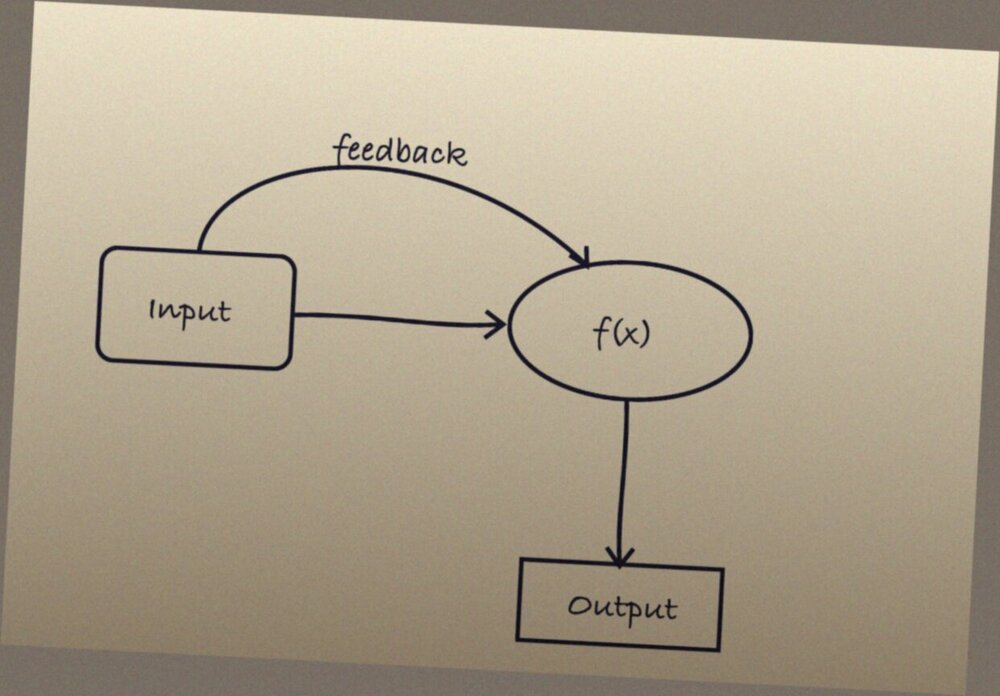
\includegraphics[width=0.36\linewidth]{img/photo.jpg}\hspace{4mm}
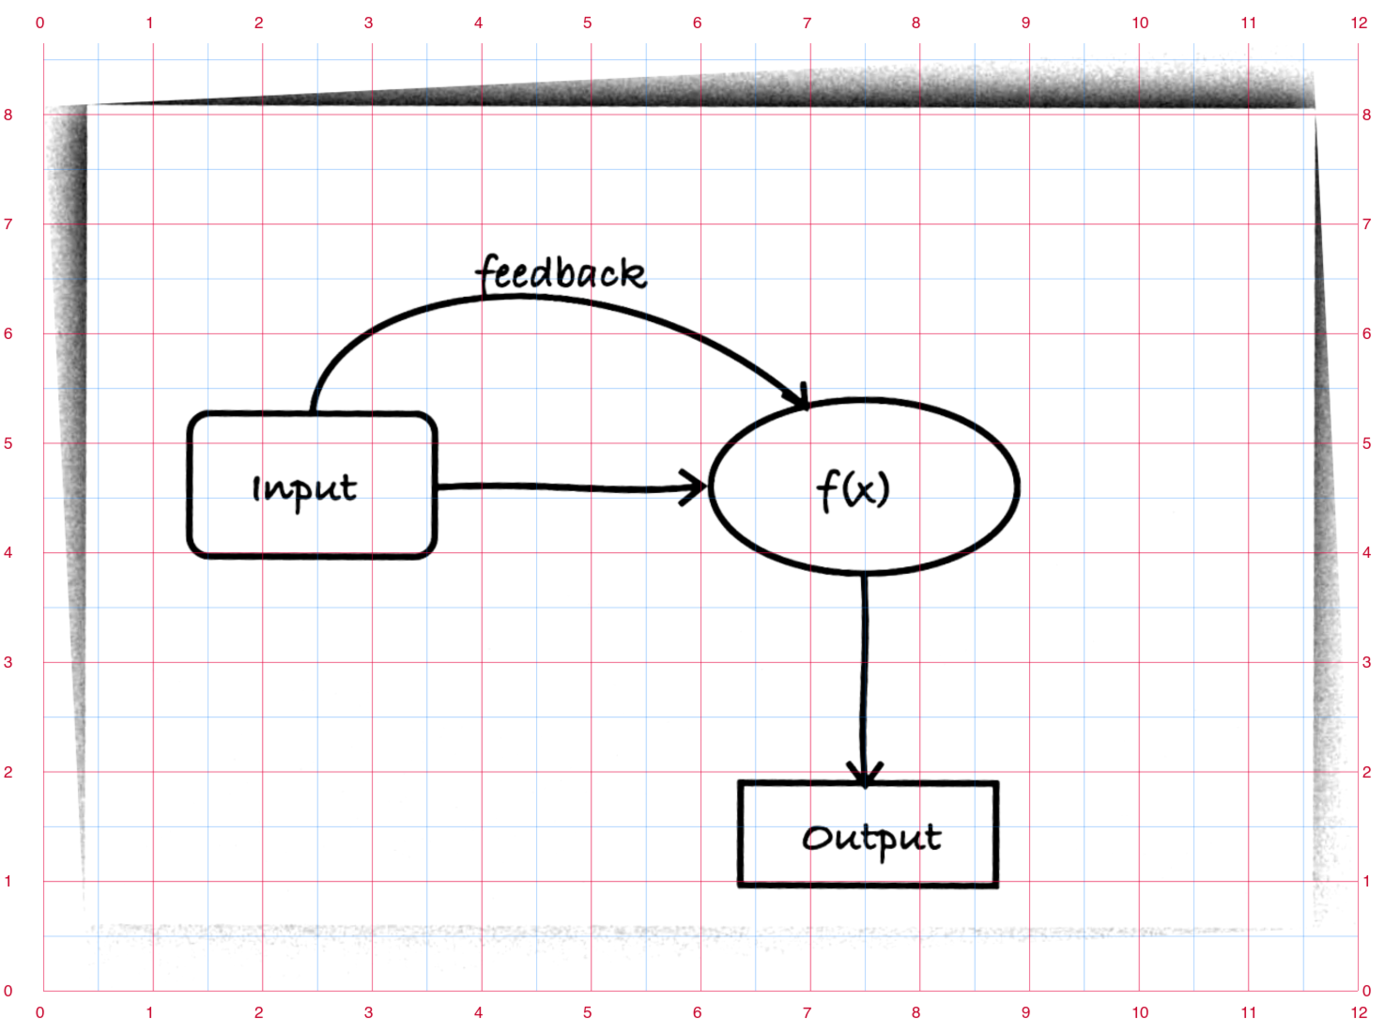
\includegraphics[width=0.52\linewidth]{img/photo-grid.png}\\[2pt]
{\small 左:入力(手書き風の写真)/右:座標グリッドを重ねた画像}
\end{center}

\paragraph{2. TikZ を書く}
グリッドで読んだ位置に、意味のある部品(ノード・スタイル・名前付き座標)として書きます。
\VerbatimInput[fontsize=\footnotesize,label={\ttfamily feedback-loop.tikz}]{img/feedback-loop.tikz}

\paragraph{3. ビルドして原図と照合する}
\begin{Verbatim}
python3 scripts/build.py feedback-loop.tikz \
        --ref work/photo-clean.png --ref-width-cm 12
\end{Verbatim}
重ね合わせ画像では、赤が原図にだけある線(描き漏れ)、青が TikZ にだけある線(余分)、
黒っぽい部分が一致です。手書きの文字と組版の文字は形が違うので、文字は位置だけを見ます。
\begin{center}
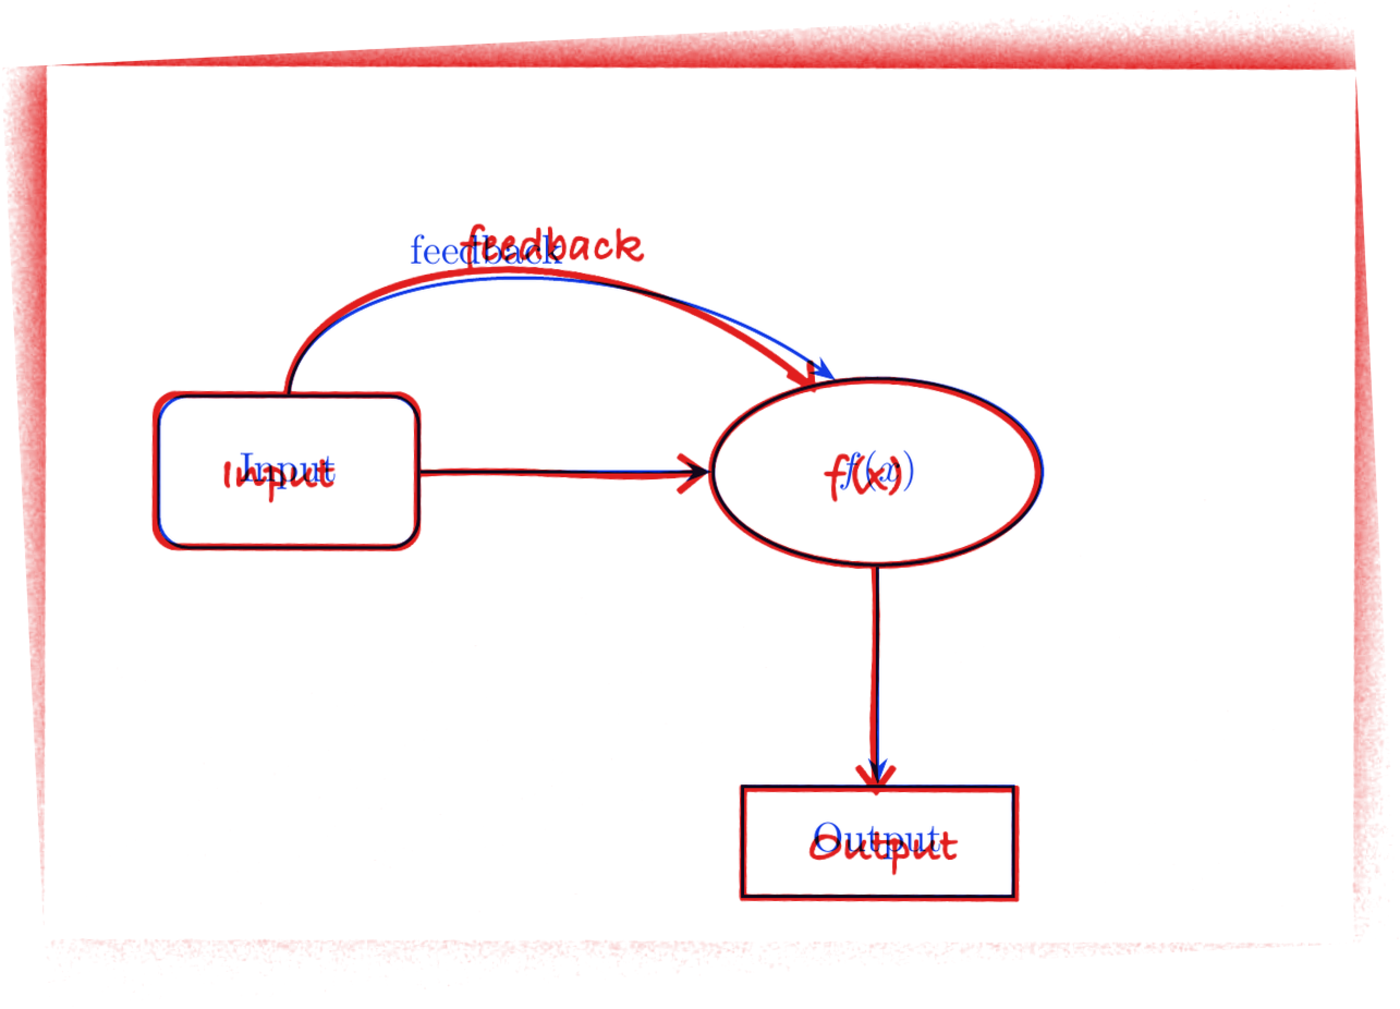
\includegraphics[width=0.62\linewidth]{img/overlay.png}\\[2pt]
{\small 重ね合わせ(赤:原図/青:TikZ)}
\end{center}

\paragraph{4. 文書に入れる}
\begin{Verbatim}
python3 scripts/insert.py --doc main.tex --fig figs/feedback-loop.tikz \
  --marker '%%FIG feedback-loop' --caption 'フィードバックループ'
\end{Verbatim}
プリアンブルに足りないパッケージだけが追記され、目印の行が次の figure 環境に置き換わります。
書き込む前に \cmd{main.tex.bak} が作られ、差分が表示されます。
\begin{Verbatim}
\begin{figure}[htbp]
  \centering
  \input{figs/feedback-loop.tikz}
  \caption{フィードバックループ}
  \label{fig:feedback-loop}
\end{figure}
\end{Verbatim}

\subsection{入力の種類と経路}
\begin{center}
\begin{tabular}{p{0.32\linewidth} p{0.58\linewidth}}
\toprule
入力 & 経路 \\
\midrule
写真・スキャン・スクショ & \cmd{grid.py} でグリッドを重ねて読む。写真は \opt{--clean} \\
SVG・PDF・EPS(ベクター) & \cmd{svg2tikz.py} で正確な座標の下書きを作り、意味的に書き直す \\
PDF に埋め込まれた画像の図 & \cmd{svg2tikz.py --crop} で画像の配置とラベル位置を取り、画像は \cmd{grid.py} で読む \\
図の元データ(Mermaid, Graphviz, draw.io, Excalidraw, matplotlib, CSV) & ソースから構造と数値を直接読む \\
PowerPoint・Keynote・Word の図 & PDF に書き出してベクター経路へ \\
\bottomrule
\end{tabular}
\end{center}

% ------------------------------------------------------------------
\section{スクリプト}
スクリプトはすべて \cmd{tikzify/scripts/} にあり、\opt{-h} で全オプションを表示します。

\subsection{grid.py --- 座標グリッド}
\begin{tabular}{>{\ttfamily}l p{0.56\linewidth}}
\toprule
\normalfont オプション & 働き \\ \midrule
--width-cm W & 画像全体の幅を W cm とみなす(仕上がり幅) \\
--dpi D & 解像度の分かるスキャンを原寸で扱う(\opt{--width-cm} の代わり) \\
--step S & 細かい目盛りの間隔(cm、既定 0.5) \\
--clean & 写真の前処理(傾き補正・影の除去・机の切り取り) \\
--frame X0,Y0,X1,Y1 & 1回目のグリッドの cm で範囲を指定して切り出す(左下が新しい原点) \\
--mask X0,Y0,X1,Y1 & 範囲を白で塗る(図番号など。複数可) \\
--zoom X0,Y0,X1,Y1 & 一部を拡大して細部を読む \\
-o OUT & 出力先(既定は元画像の隣の \texttt{work/}) \\
\bottomrule
\end{tabular}

\subsection{svg2tikz.py --- ベクター図の下書き}
\begin{tabular}{>{\ttfamily}l p{0.56\linewidth}}
\toprule
\normalfont オプション & 働き \\ \midrule
--page N & PDF のページ \\
--crop X,Y,W,H & 一部だけを変換(PDF は pt、左上原点) \\
--width-cm W & 幅 W cm に拡大縮小 \\
-o OUT.tikz & 出力先 \\
\bottomrule
\end{tabular}

\noindent PDF の文字は位置付きの \verb|\node| として取り出します。
取り出した文字は TeX の特殊文字をすべてエスケープするので、ファイルに仕込まれた
TeX コードが実行されることはありません。

\subsection{build.py --- ビルドと照合}
\begin{tabular}{>{\ttfamily}l p{0.56\linewidth}}
\toprule
\normalfont オプション & 働き \\ \midrule
--ref IMG --ref-width-cm W & 原図との重ね合わせ画像と比較画像を作る \\
--zoom X0,Y0,X1,Y1 & 重ね合わせの一部を拡大(複数可) \\
--engine E & \texttt{lualatex}(既定)/ \texttt{pdflatex} / \texttt{xelatex} \\
--doc main.tex & snippet の \verb|\input| パスを文書から見た相対パスにする \\
--caption, --label & snippet のキャプションとラベル \\
\bottomrule
\end{tabular}

\subsection{measure.py --- 画素からの実測}
\begin{tabular}{>{\ttfamily}l p{0.56\linewidth}}
\toprule
\normalfont オプション & 測るもの \\ \midrule
--row Y / --col X & その線を横切る線の位置と太さ \\
--circle X,Y,R0,R1 & 円の中心と半径(外れ値を除いて当てはめ) \\
--ellipse X,Y,R & 斜めから見た円(楕円)の中心と半径 \\
--trace X0,X1,Y0,Y1 & 曲線をなぞった点列(式の当てはめに使う) \\
--bbox X0,Y0,X1,Y1 & 文字などの塊の範囲と中心 \\
--mean X0,Y0,X1,Y1 & 塗り(網点)の濃さ → \verb|black!NN| \\
--json & 機械可読の出力 \\
\bottomrule
\end{tabular}

\subsection{insert.py --- 文書への挿入}
\begin{tabular}{>{\ttfamily}l p{0.56\linewidth}}
\toprule
\normalfont オプション & 働き \\ \midrule
--marker TEXT & その文字を含む行を figure 環境に置き換える \\
--line N & 本文の N 行目の後に入れる \\
--copy-to DIR & 図一式を文書の隣のフォルダへ複製して参照する \\
--dry-run & 差分を表示するだけで書き込まない \\
--force & 同じラベルが既にあっても入れる \\
\bottomrule
\end{tabular}

\noindent Markdown(\texttt{.md} / \texttt{.qmd})では \verb|![caption](figs/名前.svg){#fig:名前}| を挿入します。

% ------------------------------------------------------------------
\section{図の書き方の規則}
\begin{itemize}
\item \texttt{.tikz} には \verb|tikzpicture| 環境だけを書く。スタイルはピクチャの中でローカルに定義する。
\item スタイル名に TikZ の既存キー名(\texttt{in}, \texttt{out}, \texttt{at}, \texttt{label}, \texttt{node} など)を使わない。
\item フォントは指定しない(文書の書体を継承する)。大きさは \verb|\small| などの相対指定まで。
\item 数式・添字・ギリシャ文字は数式モードで書く。
\item 大きさは座標(cm)で決まる。全体を縮めるときは \verb|[x=0.8cm,y=0.8cm]| とし、\verb|scale=| や \verb|\resizebox| は避ける(文字まで縮むため)。
\item 曲線は極値・変曲点で区切り、区間ごとに1本の \verb|.. controls ..| で描く。らせんやばねは式で描く。
\end{itemize}

% ------------------------------------------------------------------
\section{テンプレート}
\cmd{tikzify/templates/} に、図の種類ごとの雛形が 12 種あります。
以下はそのファイルをそのまま \verb|\input| したものです。

\newcommand{\tpl}[2]{}
\newcommand{\tplrow}[6]{\noindent\tpl{#1}{#2}\hfill\tpl{#3}{#4}\hfill\tpl{#5}{#6}\par\bigskip}

\begingroup
\renewcommand{\tpl}[2]{%
  \begin{minipage}[b]{0.31\linewidth}\centering
  \adjustbox{max width=\linewidth,max height=3.4cm}{\input{../templates/#1.tikz}}\\[3pt]
  {\small\texttt{#1}\quad #2}
  \end{minipage}}
\tplrow{flowchart}{フローチャート}{automaton}{状態遷移}{tree}{木}
\tplrow{commutative}{可換図式}{circuit}{回路}{plot}{関数・データ}
\tplrow{bars}{棒グラフ}{geometry}{幾何}{physics}{力学}
\tplrow{timeline}{数直線}{venn}{ベン図}{solenoid}{ソレノイド}
\endgroup

% ------------------------------------------------------------------
\section{よくあるエラー}
\begin{tabular}{p{0.4\linewidth} p{0.5\linewidth}}
\toprule
メッセージ & 直し方 \\ \midrule
\texttt{Unknown arrow tip kind 'Stealth'} & \verb|\usetikzlibrary{arrows.meta}| を足す \\
\texttt{The key '/tikz/out' requires a value} & スタイル名が既存キーと衝突。名前を変える \\
\texttt{Dimension too large}(markings) & 短い線の矢じりは \verb|\draw[-{Stealth}]| で描く \\
\texttt{Missing character} & pdf\LaTeX{} で和文。Lua\LaTeX{}(luatexja)か up\LaTeX{} を使う \\
\texttt{Text line contains an invalid character} & ファイルに制御文字。エディタか \verb|printf| で書き直す \\
\verb|\input| のファイルが見つからない & パスはメインの \texttt{.tex} から見た相対パス \\
\bottomrule
\end{tabular}

\medskip
\noindent ほかの注意点は \cmd{tikzify/references/pitfalls.md} にまとめてあります。

% ------------------------------------------------------------------
\section{ライセンス}
MIT License. Copyright \copyright{} 2026 Kosei Kawaguchi.\\
\url{https://github.com/KKTeX/Publicated-Files/tree/main/tikzify}

\medskip
\noindent 図を起こす対象の著作権は元の著作者にあります。他人の図版を TikZ に起こして公開する場合は、
引用の要件や利用許諾を確認してください。

\end{document}
